\section{Buscaminas}

Descarge y pruebe
\href{../../\_static/programas/tkinter/buscaminas.py}{este programa} que
es una implementación del juego Buscaminas.

El juego consiste en descubrir las casillas de un campo minado que no
tienen minas. Al pisar una casilla que tiene una mina, se termina el
juego. El campo minado se representa como una grilla de botones:

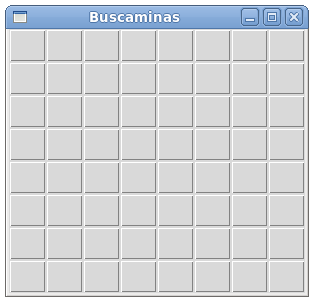
\includegraphics{../../_static/capturas/bm0.png}

Al hacer clic en una casilla no minada, aparece un número que indica en
cuántas de las ocho casillas vecinas hay una mina:

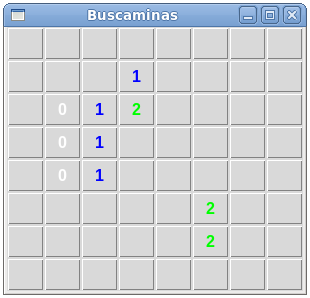
\includegraphics{../../_static/capturas/bm1.png}

Si se hace clic en una mina, el juego termina:

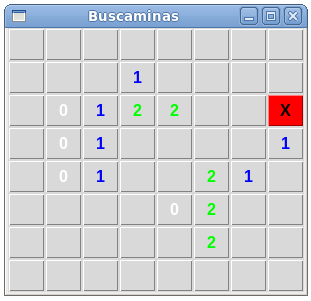
\includegraphics{../../_static/capturas/bm2.png}

\begin{enumerate}
\item
  Modifique el programa para que aparezca un mensaje en la parte
  inferior de la ventana indicando cuántas casillas no minadas faltan
  por ser descubiertas. Cada vez que se haga clic en una nueva casilla,
  el mensaje debe ser actualizado:

  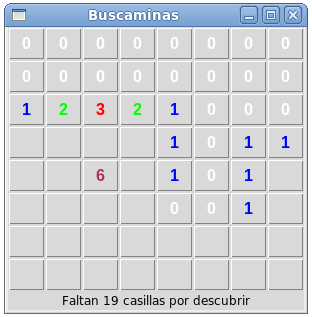
\includegraphics{../../_static/capturas/bm3.png}
\item
  Modifique el programa para que al hacer clic en una mina se muestren
  los contenidos de todas las celdas del campo minado. En la etiqueta
  inferior debe mostrarse el mensaje «¡Perdiste!». La mina que fue
  pisada debe ser indicada con una equis:

  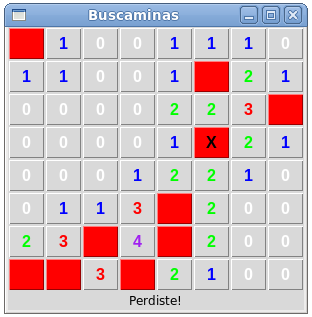
\includegraphics{../../_static/capturas/bm4.png}
\item
  Modifique el programa para que aparezca el mensaje «¡Ganaste!» cuando
  todas las casillas no minadas hayan sido descubiertas.

  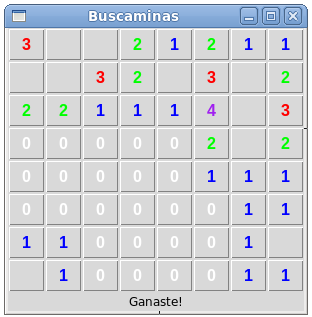
\includegraphics{../../_static/capturas/bm5.png}
\end{enumerate}
